\documentclass[unicode,11pt,a4paper,oneside,numbers=endperiod,openany]{scrartcl}
\usepackage{amsmath} % for \text command
\usepackage{ifthen}
\usepackage[utf8]{inputenc}
\usepackage{graphics}
\usepackage{graphicx}
\usepackage{hyperref}

\pagestyle{plain}
\voffset -5mm
\oddsidemargin  0mm
\evensidemargin -11mm
\marginparwidth 2cm
\marginparsep 0pt
\topmargin 0mm
\headheight 0pt
\headsep 0pt
\topskip 0pt        
\textheight 255mm
\textwidth 165mm

\newcommand{\duedate} {}
\newcommand{\setduedate}[1]{%
\renewcommand\duedate {Due date:~ #1}}
\newcommand\isassignment {false}
\newcommand{\setassignment}{\renewcommand\isassignment {true}}
\newcommand{\ifassignment}[1]{\ifthenelse{\boolean{\isassignment}}{#1}{}}
\newcommand{\ifnotassignment}[1]{\ifthenelse{\boolean{\isassignment}}{}{#1}}

\newcommand{\assignmentpolicy}{
\begin{table}[h]
\begin{center}
\scalebox{0.8} {%
\begin{tabular}{|p{0.02cm}p{16cm}|}
\hline
&\\
\multicolumn{2}{|c|}{\Large\textbf{HPC Lab for CSE 2024 ---  Submission Instructions}}\\
\multicolumn{2}{|c|}{\large\textbf{(Please, notice that following instructions are mandatory: }}\\
\multicolumn{2}{|c|}{\large\textbf{submissions that don't comply with, won't be considered)}}\\
&\\
\textbullet & Assignments must be submitted to \href{https://moodle-app2.let.ethz.ch/course/view.php?id=22516}{Moodle} (i.e. in electronic format).\\
\textbullet & Provide both executable package and sources (e.g. C/C++ files, Matlab). 
If you are using libraries, please add them in the file. Sources must be organized in directories called:\\
\multicolumn{2}{|c|}{\textit{Project\_number\_lastname\_firstname}}\\
& and  the  file must be called:\\
\multicolumn{2}{|c|}{\textit{project\_number\_lastname\_firstname.zip}}\\
\multicolumn{2}{|c|}{\textit{project\_number\_lastname\_firstname.pdf}}\\
\textbullet &  The TAs will grade your project by reviewing your project write-up, and looking at the implementation 
                 you attempted, and benchmarking your code's performance.\\

\textbullet & You are allowed to discuss all questions with anyone you like; however: (i) your submission must list anyone you discussed problems with and (ii) you must write up your submission independently.\\
\hline
\end{tabular}
}
\end{center}
\end{table}
}
\newcommand{\punkte}[1]{\hspace{1ex}\emph{\mdseries\hfill(#1~\ifcase#1{Points}\or{Points}\else{Points}\fi)}}


\newcommand\serieheader[6]{
\thispagestyle{empty}%
\begin{flushleft}

\includegraphics[width=0.4\textwidth]{ETHlogo_13}
\end{flushleft}
  \noindent%
  {\large\ignorespaces{\textbf{#1}}\hspace{\fill}\ignorespaces{ \textbf{#2}}}\\ \\%
  {\large\ignorespaces #3 \hspace{\fill}\ignorespaces #4}\\
  \noindent%
  \bigskip
  \hrule\par\bigskip\noindent%
  \bigskip {\ignorespaces {\Large{\textbf{#5}}}
  \hspace{\fill}\ignorespaces \large \ifthenelse{\boolean{\isassignment}}{\duedate}{#6}}
  \hrule\par\bigskip\noindent%  \linebreak
 }

\makeatletter
\def\enumerateMod{\ifnum \@enumdepth >3 \@toodeep\else
      \advance\@enumdepth \@ne
      \edef\@enumctr{enum\romannumeral\the\@enumdepth}\list
      {\csname label\@enumctr\endcsname}{\usecounter
        {\@enumctr}%%%? the following differs from "enumerate"
	\topsep0pt%
	\partopsep0pt%
	\itemsep0pt%
	\def\makelabel##1{\hss\llap{##1}}}\fi}
\let\endenumerateMod =\endlist
\makeatother




\usepackage{textcomp}






\begin{document}


\setassignment
\setduedate{Monday 20 May 2024, 23:59}

\serieheader{AI in the Sciences and Engineering}{Spring Semester 2024}
            {Student: Carla Judith L\'opez Zurita}
            {}{Project 2}

The main objective of the project is to apply the concepts learned in class
related to Neural Operators. 
The first task consists in making future (or out of samples) predictions of the fluid and solid
temperature of a thermal storage system. The second task is to model the water
flow on the sphere using a
Spherical Fourier Neural Operator (SFNO) and compare the results with the ones
obtained by a baseline neural operator.
The project also includes an optional task to test the universal approximation
property of the Convolutional Neural Operator (CNO).
My attempt at solving each of the mentioned tasks will be described in detail below.


\section{Time Series Forecasting with Neural Operators}\label{sec:task1}
The first task is based on the mathematical model of a thermal storage system
described by the following PDEs:
\begin{align}
    \epsilon \rho_f C_f \frac{\partial T_f}{\partial t} + \epsilon \rho_f C_f u_f(t) \frac{\partial T_f}{\partial x} = \lambda_f \frac{\partial^2 T_f}{\partial x^2} - h_v(T_f - T_s) \quad \text{for} \quad x \in [0, L], \quad t \in [0, T],
    \\
    (1-\epsilon)\rho_s C_s\frac{\partial T_s}{\partial t} = \lambda_s \frac{\partial^2 T_s}{\partial x^2} + h_v(T_f - T_s) \quad \text{for} \quad x \in [0, L], \quad t \in [0, T],
\end{align}
with $\rho$ being the density of the phases, $C$ the specific heat, $\lambda$ the diffusivity, $\epsilon$ the solid porosity, $u_f$
the fluid velocity entering the thermal storage and $h_v$ the heat exchange
coefficient between solid and fluid.
The system is also defined with appropriate boundary conditions defined in the
project description.
The goal is to predict the fluid and solid temperature at future time steps
using a Neural Operator.
One of the main challenges of this task was to arrange the data in the correct
format to feed it to the network, namely the data had to be arranged in a
series of windows. I used a window generator to create the windows with a length
of 34 for both inputs and outputs, which was chosem because it is the size of the
final prediction we have to make. 
The outputs were taken from the provided measurements, but corresponding to the
next 34 time steps. Fig. \ref{fig:window} shows an example of a window with
prediction.
\begin{figure}[ht!]
    \centering
    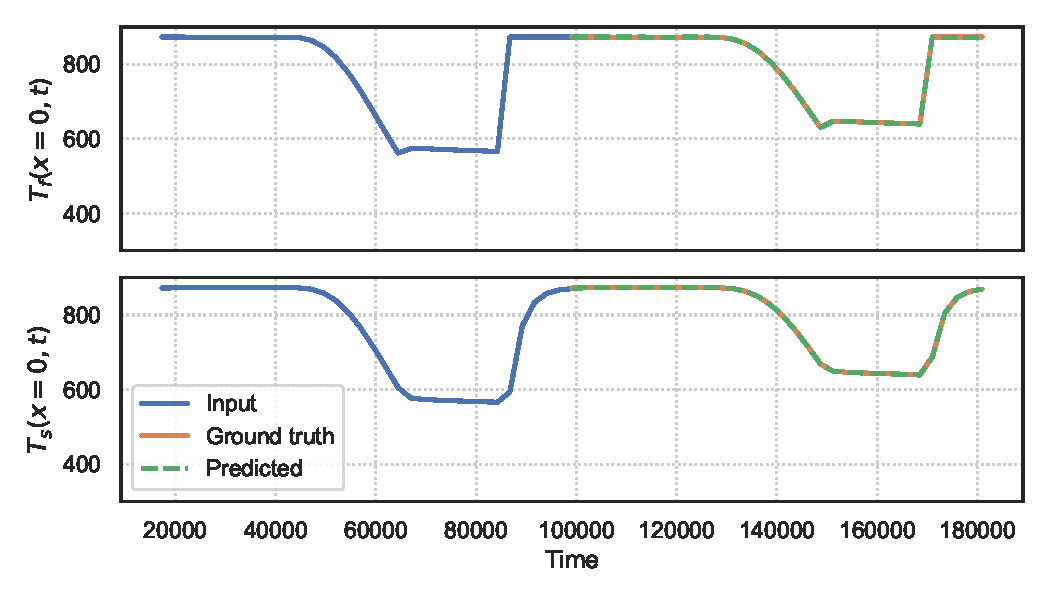
\includegraphics[width=0.8\textwidth]{../task1/fno/plot_window_5.pdf}
    \caption{Example of a window with prediction.}
    \label{fig:window}
\end{figure}

The data was normalized using the MinMaxScaler from the sklearn library.
The data was split into training and validation sets with a
ratio of 80\% and 20\% respectively.
I chose to use a Fourier Neural Operator (FNO) to solve this task. I used a
single network to predict both the fluid ($T_f$) and solid temperature ($T_s$),
so that it had three
channels as input ($T_f$, $T_s$ and time) and two channels as output ($T_f$ and
$T_s$). 
The network
consisted of 3 layers with 3 Fourier features each.
It was trained using the Adam optimizer with an initial learning rate
of $10^{-3}$ and a batch size of 10. The loss function used was the L2 norm. The
network was trained for 500 epochs.
The loss function of the model during training is shown in Fig. \ref{fig:loss}.
\begin{figure}[ht!]
    \centering
    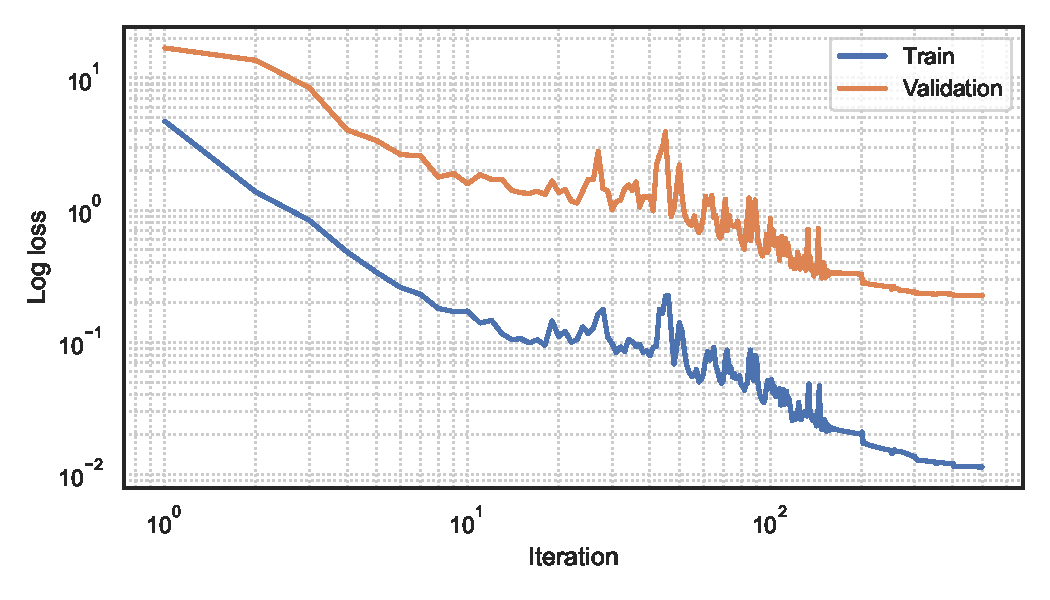
\includegraphics[width=0.8\textwidth]{../task1/fno/loss_function.pdf}
    \caption{Loss function of the FNO model during training.}
    \label{fig:loss}
\end{figure}

The model was evaluated on the test set and the predictions were compared with
the ground truth. Fig. \ref{fig:predictions} shows the predictions of the model
taken from various windows in the test set. The dashed lines represent the
predicted values, while the solid lines depict the ground truth.
The model seems to be able to capture the general trend of the data, and predict
very close values.
\begin{figure}[ht!]
    \centering
    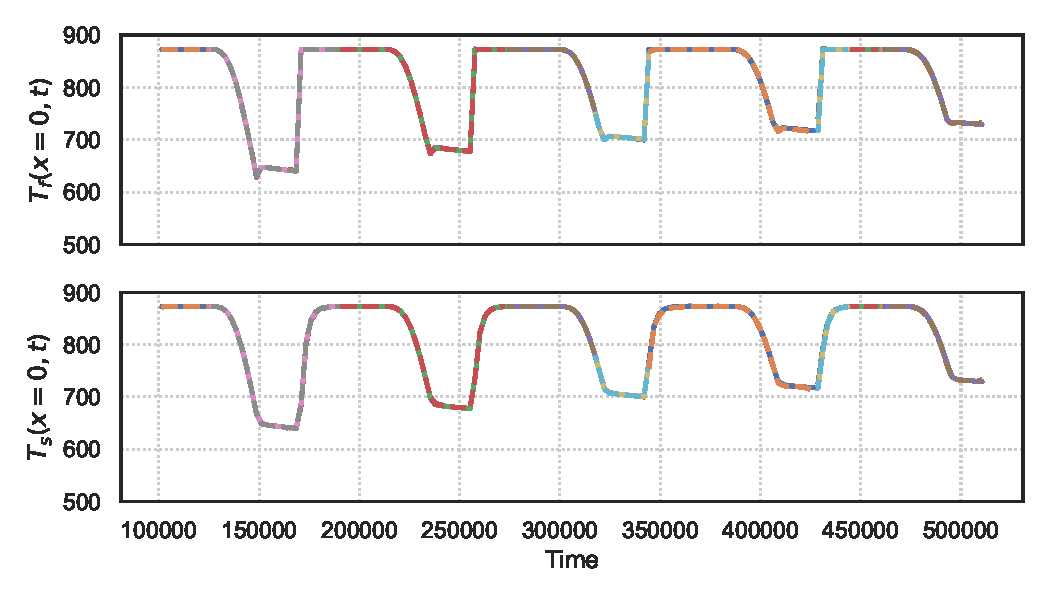
\includegraphics[width=0.8\textwidth]{../task1/fno/plot_predictions.pdf}
    \caption{Predictions of the FNO model taken from various windows in the test set. Dashed lines represent the predicted values, solid lines depict ground truth.}
    \label{fig:predictions}
\end{figure}

Finally, we show the future predictions of the fluid and solid temperature in
Fig. \ref{fig:future}.
\begin{figure}[ht!]
    \centering
    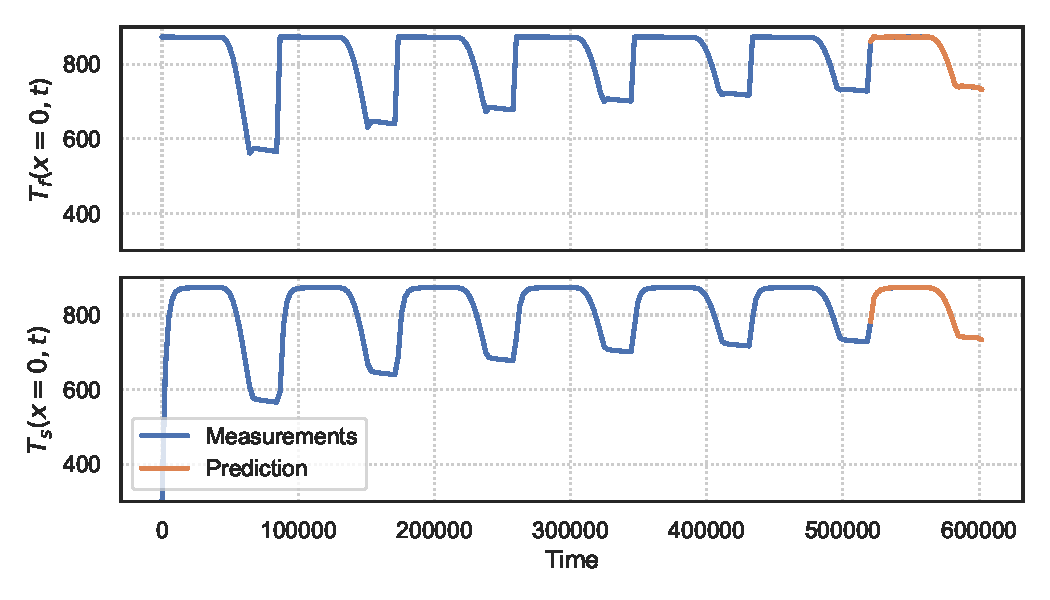
\includegraphics[width=0.8\textwidth]{../task1/fno/plot_complete.pdf}
    \caption{Future predictions of the fluid and solid temperature.}
    \label{fig:future}
\end{figure}

\section{Modeling Water Flow on the Sphere with FNO}\label{sec:task2}
The next task consists in modeling the water flow on the sphere using a
Spherical
Fourier Neural Operator (SFNO) and comparing the results with the ones obtained
by a baseline neural operator.


\section{Universal Approximation for CNO (Optional)}\label{sec:task3}

\bibliographystyle{plain}
\bibliography{bibliography}

\end{document}
